%%%%%%%%%%%%%%%%%%% JAVA SCRIPT SUPPORT %%%%%%%%%%%%%%%%%%%%%%%%
\definecolor{lightgray}{rgb}{.9, .9, .9}
\definecolor{darkgray}{rgb}{.4, .4, .4}
\definecolor{purple}{rgb}{0.65, 0.12, 0.82}

\lstdefinelanguage{JavaScript}{
        keywords={typeof, new, true, false, catch, function, return, null, catch, switch, var, if, in, while, do, else, case, break},
        keywordstyle=\color{blue}\bfseries,
        ndkeywords={class, export, boolean, throw, implements, import, this},
        ndkeywordstyle=\color{darkgray}\bfseries,
        identifierstyle=\color{black},
        sensitive=false,
        comment=[l]{//},
        morecomment=[s]{/*}{*/},
        commentstyle=\color{purple}\ttfamily,
        stringstyle=\color{red}\ttfamily,
        morestring=[b]',
        morestring=[b]"
        }


\section{Implementierung}
\subsection*{}
\begin{frame} 
  \frametitle{Suchfunktion im Überblick}
  \begin{figure}[htbp]
\centering
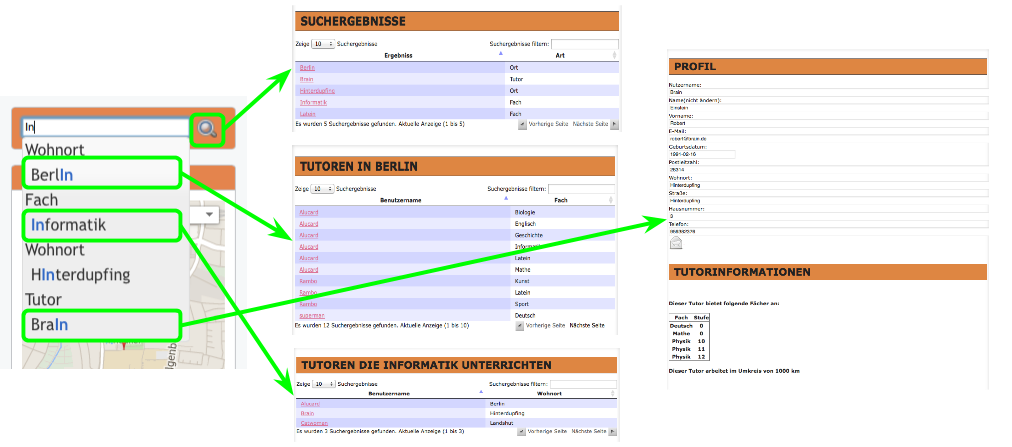
\includegraphics[width=1.0\textwidth]{./chapters/SufuOverview.png}
\caption{Suchfunktion}
\label{fig:SufuOverview}
\end{figure}

\end{frame}

\subsection{Clientseitige Implementierung}

\defverbatim[colored]
\makeset{
\lstset{
        language=JavaScript,
        backgroundcolor=\color{lightgray},
        extendedchars=true,
        basicstyle=\tiny\ttfamily,
        showstringspaces=false,
        showspaces=false,
        numbers=left,
        numberstyle=\tiny\ttfamily,
        numbersep=9pt,
        tabsize=2,
        breaklines=true,
        showtabs=false,
        frame=leftline,
        literate={\$}{{\textcolor{blue}{\$}}}1,
        mathescape=false
        }

\begin{lstlisting}[name = Autocomplete.js]
$(function() {
    $('[name="search"]').catcomplete({
        source: "/scripts/autocomplete.php",
        minLength: 2,
        select: function(event, ui) {
            var url = ui.item.id;
            var value = ui.item.value;
            var typ = ui.item.typ;
            if (url != '#') {
                $('[name="search"]').val(value);
                $('[name="valueTyp"]').val(typ);
                $('#searchform').attr('action', url);
                $('#searchform').submit();
            }
        }
    });
});
\end{lstlisting}
}

\begin{frame} 
  \frametitle{JS, Ajax, jQuery}
  \makeset
\end{frame}

\defverbatim[colored]
\makeset{
%%%%%%%%%%%%%%%%%%% PHP SUPPORT %%%%%%%%%%%%%%%%%%%%%%%%
\definecolor{dkgreen}{rgb}{0,.6,0}
\definecolor{dkblue}{rgb}{0,0,.6}
\definecolor{dkyellow}{cmyk}{0,0,.8,.3}

\lstset{
  language        = php,
  backgroundcolor=\color{lightgray},
  extendedchars=true,
  basicstyle=\tiny\ttfamily,
  showstringspaces=false,
  showspaces=false,
  numbers=left,
  numberstyle=\tiny\ttfamily,
  numbersep=9pt,
  tabsize=2,
  breaklines=true,
  showtabs=false,
  frame=leftline,
  keywordstyle    = \color{dkblue},
  stringstyle     = \color{red},
  identifierstyle = \color{dkgreen},
  commentstyle    = \color{gray},
  emph            =[1]{php},
  emphstyle       =[1]\color{black},
  emph            =[2]{if,and,or,else},
  emphstyle       =[2]\color{dkyellow}
  }
  
\begin{lstlisting}[name=Autocomplete.php]
  <?php
$term = trim($_GET['term']);
$conn = ConnectToDB();
$sql = "SELECT * FROM suche WHERE (Wohnort LIKE '" . $term . "%') or (fach LIKE '" . $term . "%') or (benutzername LIKE '" . $term . "%')";
$sth = $conn->prepare($sql);
$sth->execute();
while ($row = $sth->fetch(PDO::FETCH_ASSOC)) {
    if (stristr($row['Wohnort'], $term)) {
        $a_json_row["id"] = "/de/search.php";
        $a_json_row["value"] = $row['Wohnort'];
        $a_json_row["typ"] = "location";
        array_push($a_json, $a_json_row);}
    if (stristr($row['benutzername'], $term)) {
        $a_json_row["id"] = "/de/profile.php?username=" . $row['benutzername'];
        $a_json_row["value"] = $row['benutzername'];
        $a_json_row["typ"] = "user";
        array_push($a_json, $a_json_row); }
    if (stristr($row['fach'], $term)) {
        $a_json_row["id"] = "/de/search.php";
        $a_json_row["value"] = $row['fach'];
        $a_json_row["typ"] = "subject";
        array_push($a_json, $a_json_row);}}
$a_json = array_unique($a_json, SORT_REGULAR);
$json = json_encode($a_json);
print $json;
?>
\end{lstlisting}
}

\subsection{Serverseitige Implementierung}

\begin{frame} 
  \frametitle{PHP, PDO, SQL}
  \makeset
\end{frame}

\defverbatim[colored]
\makeset{
%%%%%%%%%%%%%%%%%%% PHP SUPPORT %%%%%%%%%%%%%%%%%%%%%%%%
\definecolor{dkgreen}{rgb}{0,.6,0}
\definecolor{dkblue}{rgb}{0,0,.6}
\definecolor{dkyellow}{cmyk}{0,0,.8,.3}

\lstset{
  language        = php,
  backgroundcolor=\color{lightgray},
  extendedchars=true,
  basicstyle=\tiny\ttfamily,
  showstringspaces=false,
  showspaces=false,
  numbers=left,
  numberstyle=\tiny\ttfamily,
  numbersep=9pt,
  tabsize=2,
  breaklines=true,
  showtabs=false,
  frame=leftline,
  keywordstyle    = \color{dkblue},
  stringstyle     = \color{red},
  identifierstyle = \color{dkgreen},
  commentstyle    = \color{gray},
  emph            =[1]{php},
  emphstyle       =[1]\color{black},
  emph            =[2]{if,and,or,else},
  emphstyle       =[2]\color{dkyellow}
  }
  
\begin{lstlisting}[name=Autocomplete.php]
  <?php  /* Code reduziert, Abfrage an Datenbank mit Suchterm */
  if (count($a_json) === 1) {
    if ($a_json[0]['typ'] == "Ort") {
        $id = $a_json[0]['value'];
        header("Location: http://ebenezer-kunatse.net/de/location.php?term=$id"); exit;
    } else if ($a_json[0]['typ'] == "Fach") {
        $id = $a_json[0]['value'];
        header("Location: http://ebenezer-kunatse.net/de/subject.php?term=$id"); exit;
    } else if ($a_json[0]['typ'] == "Tutor") {
        $id = $a_json[0]['value'];
        header('Location: http://ebenezer-kunatse.net' . $a_json[0]['url']); exit; }
} else {
    include_once($_SERVER["DOCUMENT_ROOT"] . "/test_02/scripts/session.php");       
    $titel = "Suchergebnisse";
    $_SESSION['sprache'] = "de";
    include($_SERVER["DOCUMENT_ROOT"] . "/test_02/layout/header.php");
    ?>
    <script type="text/javascript">
            var searchresults = <?php echo $json; ?>;
    </script>
<?php
    include_once($_SERVER["DOCUMENT_ROOT"] . "/test_02/de/content/search.html");
    include($_SERVER["DOCUMENT_ROOT"] . "/test_02/layout/footer.php"); }
?>
\end{lstlisting}
}

\subsection{Intelligente Weiterleitung}

\begin{frame} 
  \frametitle{Intelligente Weiterleitung}
  \makeset
\end{frame}

\subsection*{}
\begin{frame}
  \frametitle{Demonstration}
  \textbf{Es folgt eine Demonstration ...}
\end{frame}